% Chapter 3

\chapter{The Maxillo Dataset}

\lhead{Chapter 3. \emph{The Maxillo Dataset}} % This is for the header on each page - perhaps a shortened title
\label{chp:maxillo}
%----------------------------------------------------------------------------------------

\def\:{\hskip0pt} %Definisce un modo veloce per permettere a latex di sillabare correttamente anche parole come 4-connectivity. Il corretto utilizzo è il seguente: 4\:-\:connectivity.

\section{Introduction}
Nowadays, perfect anatomical annotation accuracy is usually not achieved, in
favor of a fast execution time. A sparse annotation (Fig. \ref{fig:2dannot}),
performed on a 2D image, can be realized in a relatively small amount of time,
and has become the de facto standard in radiologic medical centers for dentistry
and maxillofacial purposes (a specialty also known as dento-maxillofacial
radiology). However, 2D annotations lack a considerable amount of inner
information about the bone structure and the IAN position. Surgeons rely on a
partial and incomplete idea of nerve positioning, which is generally sufficient
for a positive outcome of surgical intervention but does not represent an
accurate anatomical representation. Switching to 3D annotations (Fig.
\ref{fig:3dannot}) solves the issue, but raises the costs in terms of working
time: the manual segmentation of a single scan volume, depending on the
available software, can take hours. Therefore, although dento-maxillofacial
radiology would largely benefit from 3D annotated patients, any manual method
currently appears unsuitable for practical applications.

\begin{figure}
  \centering
  \begin{subfigure}{.35\textwidth}
    \centering
    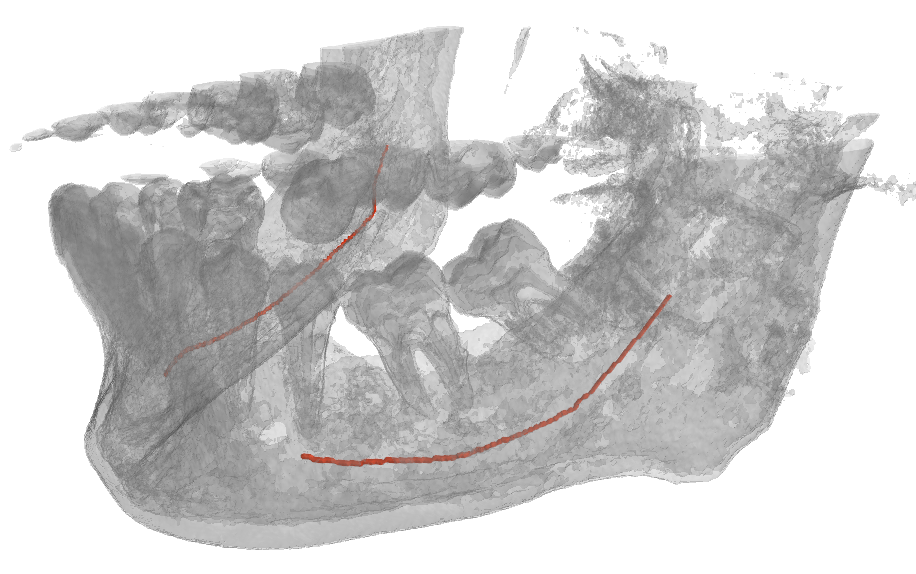
\includegraphics[width=\textwidth]{Images/sparse_annotation.png}
    \caption{2D annotation.}
    \label{fig:2dannot}
  \end{subfigure}
  \begin{subfigure}{0.35\textwidth}
    \centering
    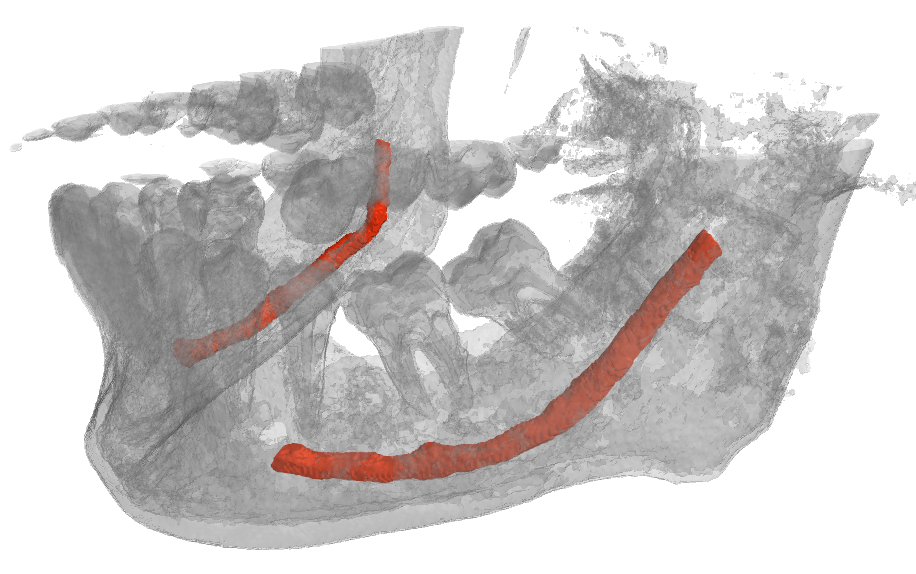
\includegraphics[width=\textwidth]{Images/dense_annotation.png}
    \caption{3D annotation.}
    \label{fig:3dannot}
  \end{subfigure}
  \caption{2D and 3D annotations of the same patient.}
  \label{fig:2d3dannot}
\end{figure}

An additional constraint when dealing with the medical branch of deep learning
regards the extra consideration for sensitive data, which must always be taken
into account. Medical data contain a huge amount of personal information which
must be protected through data anonymization. Besides the sensible details about
the patient, generally stored in the DICOM format, when it comes to medical
imaging, the personal features of one subject can be inherently carried by the
images. Therefore, in order to evaluate the correctness of the anonymization
steps and the security of the information, every medical dataset must undergo
evaluation of specific committees. Several bureaucratic steps generally stand
before the official release to the scientific community. This circumstance,
combined with the laws of individual countries, creates a serious burden for the
spread of medical datasets and makes any contribution valuable. For those
reasons, deep learning works applied to medical imaging — and in particular, to
the maxillofacial field— are often based on private internal datasets. Despite
any alleged intention, datasets are rarely released after publication, creating
a vast information gap for the research community: researchers are unable to
replicate experiments and lack valid benchmarks for their novelties.

\section{Dataset}
Cipriano et al. \cite{cipriano2022deep} have released a public dataset of
maxillofacial scans with a sparse and deep labels, which is the first of its
kind.
The 3D CBCT volumes composing the dataset have been acquired by the Affidea
center located in Modena, Italy. Affidea is a leading pan-European healthcare
group specialized in the provision of advanced diagnostics, specialist
outpatient services, laboratory analyses, physiotherapy and rehabilitation,
cancer diagnosis, and treatment. It counts $312$ different centers in $15$
different countries, with about 11 000 professionals. The dataset counts $347$
dental scans obtained by means of Cone Beam Computed Tomography
(\texttt{NewTom/NTVGiMK4, 3 mA, 110 kV, 0.3 mm cubic voxels}). Pixel spacing and
intra-slice distance are always $0.3$ millimeters. Data volumes are already
converted to the Hounsfield Unit (HU) and their values range between $-1000$ and
$5264$. During the conversion to HU we also took care of the proper processing
for the window width and center according to the DICOM format. Volume shapes
range from $(148, 265, 312)$ to $(178, 423, 463)$ for the \texttt{Z}, \texttt{Y}
and \texttt{X} axes respectively. Every patient was anonymized, hence we were
only able to access a few personal details - namely gender, age, and year of the
scan. Specifically, 59\% of the patients are female, all the scans were
performed between 2019 and 2020, and volumes belong to patients with ages in the
range $(10-100]$ with the highest frequencies in ranges $(20-30]$ and $(60-70]$.

\subsection{2D sparse annotations}
Technicians involved in the diagnostic exam were also responsible for the
original sparse annotation of the mandibular canal. This annotation performed on
2D panoramic views of the jawbone is employed in everyday surgical practice to
measure the height and depth of the sites where the implant must be placed,
avoiding inferior alveolar nerve injuries. In these labels, the upper bound of
the canal is marked along the entire dental arch, providing a useful sparse
approximation trace of nerve position. Particularly, the annotation process
starts from an axial slice (Fig. \ref{fig:axial-slice} of the original volume.
Upon this slice, a spline is manually drawn to fit the central part of the
jawbone.

\begin{figure}[ht]
  \centering
  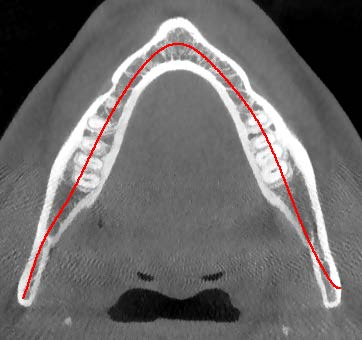
\includegraphics[width=0.45\textwidth]{Images/axial-slice.jpg}
  \caption{Axial slice.}
  \label{fig:axial-slice}
\end{figure}

This spline, called the panoramic base curve, is then employed for generating
the panoramic view (Fig. \ref{fig:panoramic}) composed by the voxels of the
curved plane identified by the base curve and orthogonal to the axial slice.
From this view, the inferior alveolar nerve canal should be clearly identifiable
and can be annotated as in Fig. \ref{fig:panoramic_annotated}.

\begin{figure}[!ht]
  \centering
  \begin{subfigure}{0.8\textwidth}
    \centering
    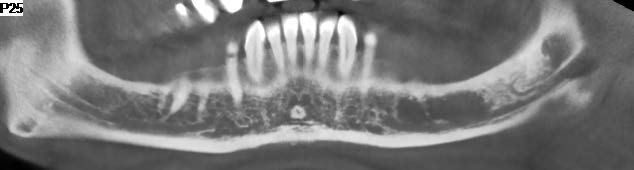
\includegraphics[width=\textwidth]{Images/panoramic.jpg}
    \caption{Panoramic view obtained from the spline drawn on the axial slice.}
    \label{fig:panoramic}
  \end{subfigure}

  \begin{subfigure}{0.8\textwidth}
    \centering
    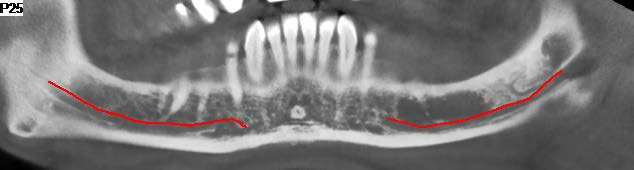
\includegraphics[width=\textwidth]{Images/panoramic_annotated.jpg}
    \caption{Panoramic view with the inferior alveolar nerve canal annotated in
    red.}
    \label{fig:panoramic_annotated}
  \end{subfigure}
  \caption{Panoramic view and its annotation.}
  \label{fig:2d3dannot}
\end{figure}

\subsection{3D dense annotations}
In order to obtain finely-grained annotations, a team of doctors with years of
experience in maxillofacial surgery elaborated $91$ volumes to produce dense
voxel-level annotations of the canal. The proposed dataset of $347$ scans is
therefore divided into two partitions: the primary dataset, composed of the $91$
volumes for which both dense and sparse annotations are available, and the
secondary dataset, only sparsely annotated.

The entire voxel-level annotation procedure has been performed by means of a
tool developed by Mercadante et al. \cite{mercadante2021cone} which allowed to
drastically reduce the burden necessary to produce the 3D label.
The annotation steps can be summarized as follows:
\begin{enumerate}
  \item{After loading the input data, the arch approximation that better
    describes the canal course is identified inside one of the axial images and
    manually adjusted. The output is a one-pixel thick curve crossing the dental
    arch which is approximated with a polynomial. The result is similar to the
    one in Fig. \ref{fig:axial-slice}, but this time it is automatically
    generated and manually adjusted only if needed.}

  \item{Sampling the polynomial, the tool thus generates a Catmull-Rom spline.
    For each point of the spline, a perpendicular line (lying on the axial
    plane) is computed (Fig. \ref{fig:csl}). These lines are called
    Cross-Sectional Lines or CSLs in short. Here, a different resolution of the
    spline generates more or fewer CSLs. This represents a crucial step for
    having a complete annotation of the mandibular canal. Indeed, with a short
    spline, some regions of the jawbone, especially near the mandibular foramen,
    would be excluded from the next stages.}

  \item{CSLs are the base of Multi Planar Reformations(MPRs) called
    Cross-Sectional Views (CSVs). These views are 2D images obtained
    interpolating the values of the respective baselines (CSL) across the whole
    volume height. As an example, the blue plane reported in Fig.
    \ref{fig:csl-orthogonal} is a Cross-Sectional Plane (CSP) generating a
    cross-sectional View. CSPs are additionally rotated around the CSLs, to have
    CSVs orthogonal to the canal slope.}

  %TODO Fig 6
  \item{For each CSV, a closed Catmull-Rom spline is finally drawn to annotate
    the position of the IAC (green lines of Fig. 6).}

  \item{The splines are saved as the coordinates of their control points. The
    final smooth and precise ground-truth volume constituting the dataset is
    generated from this set of points by means of the \textalpha-shape algorithm
    \cite{edelsbrunner1983shape}, which is described in detail in the Section
    \ref{sec:alpha}.}
\end{enumerate}

\begin{figure}[!ht]
  \centering
  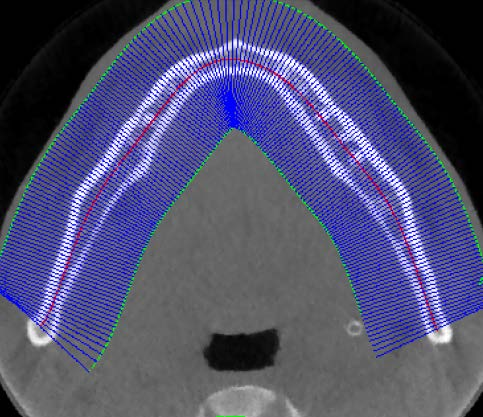
\includegraphics[width=0.45\textwidth]{Images/csl.jpg}
  \caption{Cross-Sectional Lines.}
  \label{fig:csl}
\end{figure}

\begin{figure}[!ht]
  \centering
  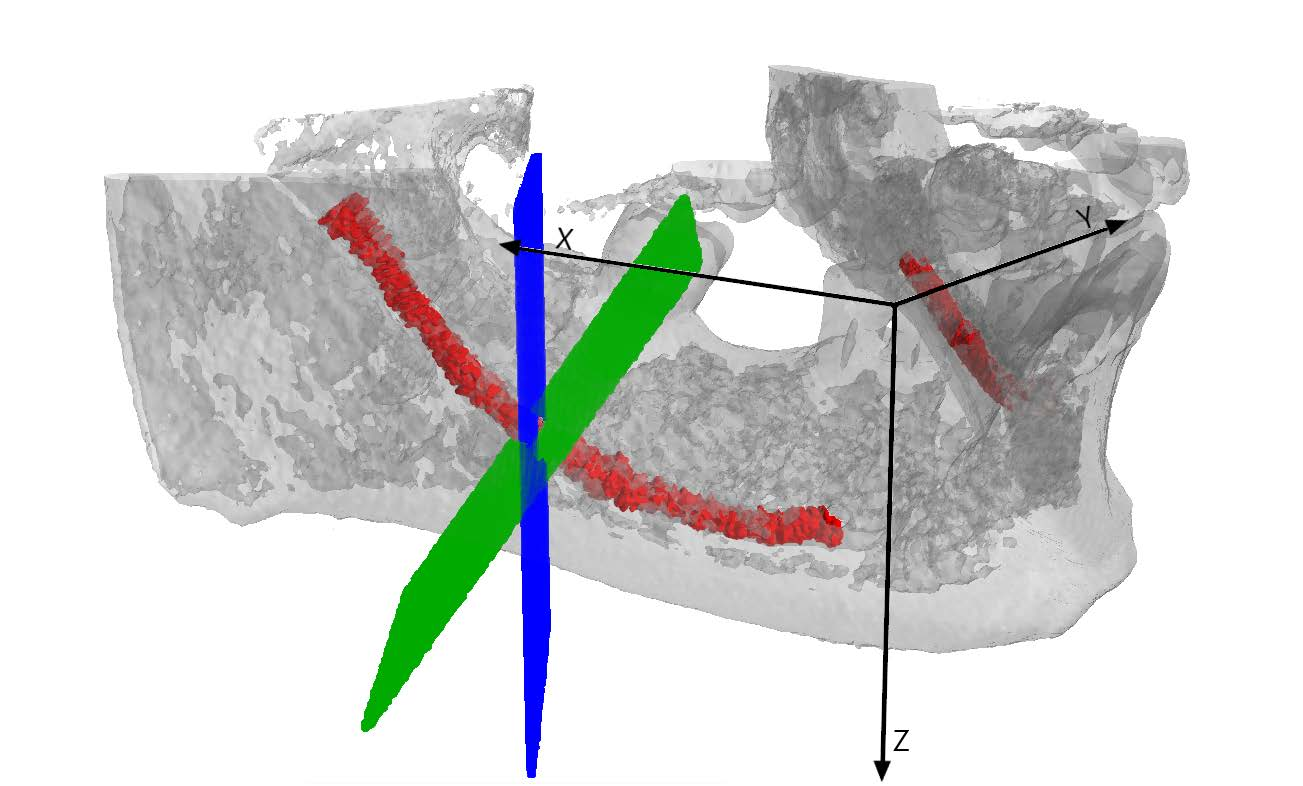
\includegraphics[width=0.5\textwidth]{Images/csl-orthogonal.jpg}
  \caption{Cross-Sectional Lines.}
  \label{fig:csl-orthogonal}
\end{figure}

Comparing the two procedures, it is possible to see that while sparse
annotations are quick and easy to obtain, creating dense labels from 3D volumes
is a very tedious and time-consuming process. For this reason, researchers
typically have few dense annotations available and preserve them as the test
set. Indeed, densely annotated volumes must always be used in tests, to ensure a
real medical feedback on model performance.

\subsection{Pre-processing with \textalpha-shape}
\label{sec:alpha}
The hand-drawn ground truth annotations produced with the tool described in the
previous section result in a dense and jagged point set; an example is depicted
in Fig. \ref{fig:pointset}. Starting from this point set, we reconstruct a
smoother polygon mesh in the form of the \textalpha-shape. The \textalpha-shape,
defined by Edelsbrunner et al. is a generalization of the concept of the convex
hull, useful to capture the intuitive notion of the shape of a point set. The
definition refers to the 2-dimensional case, but the extension to point sets in
$k$ dimensions is straightforward. The \textalpha-shape is parameterized over
$\alpha \in \mathbb{R}$, which determines the "crudeness`` of the result.\\

\begin{figure}[t]
  \centering
  \begin{subfigure}{.45\textwidth}
    \centering
    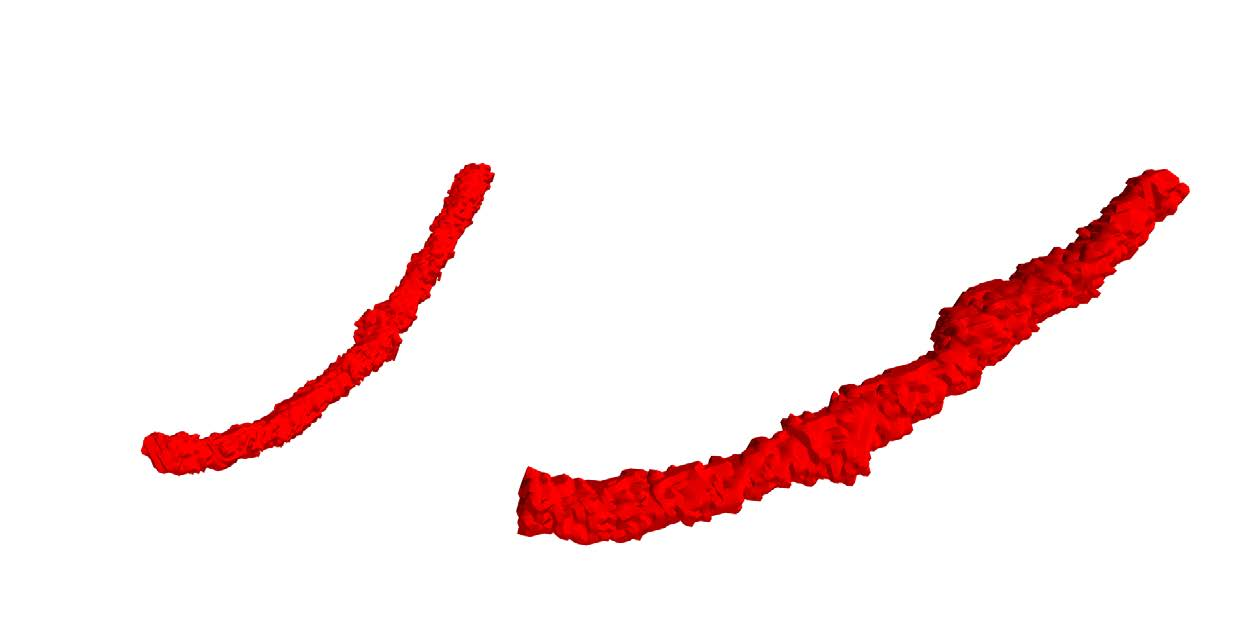
\includegraphics[width=\textwidth]{Images/pointset.jpg}
    \caption{Jagged point set.}
    \label{fig:pointset}
  \end{subfigure}
  \begin{subfigure}{0.45\textwidth}
    \centering
    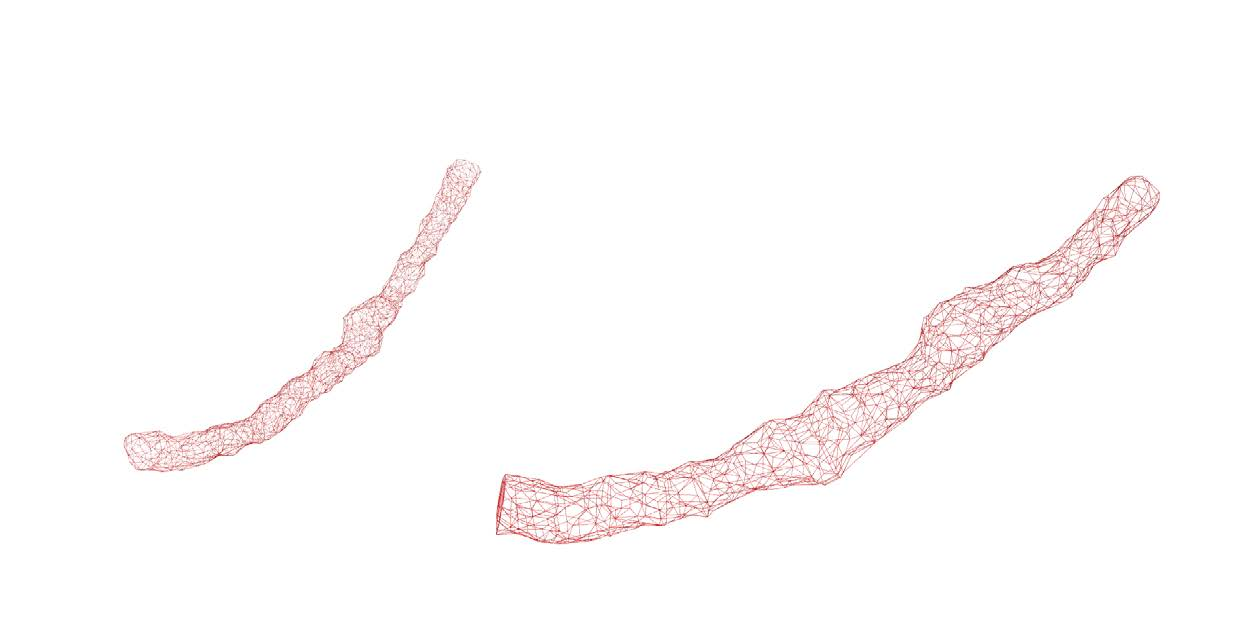
\includegraphics[width=\textwidth]{Images/alpha1.jpg}
    \caption{\textalpha-shape mesh.}
    \label{fig:alpha1}
  \end{subfigure}
  \begin{subfigure}{0.45\textwidth}
    \centering
    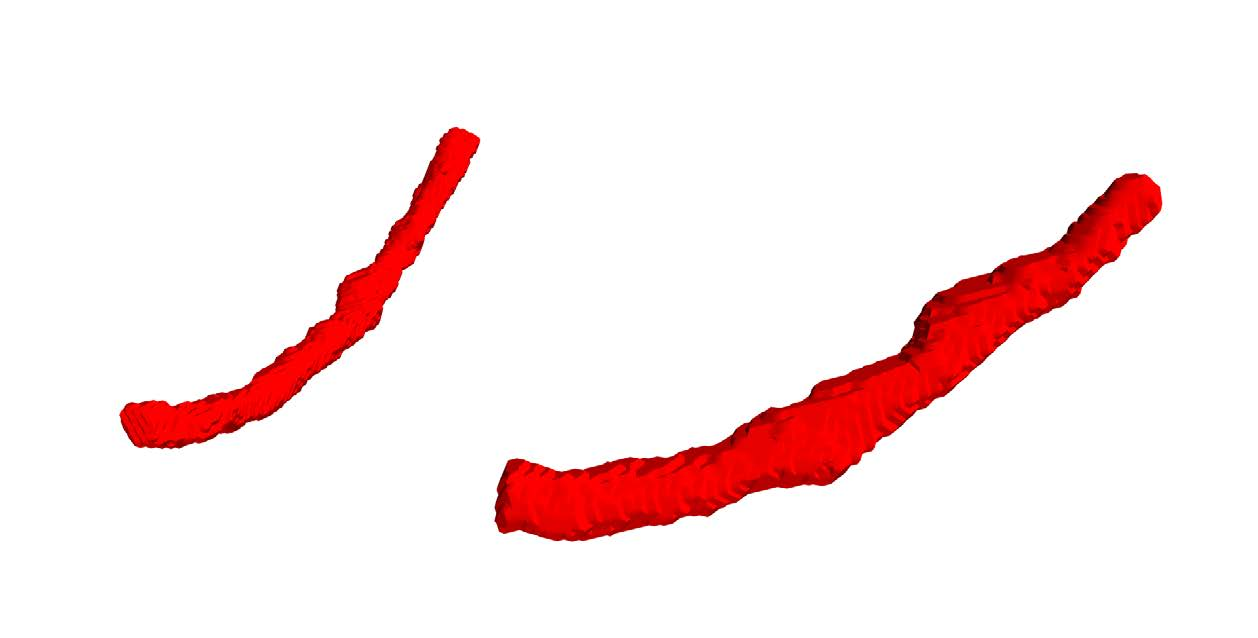
\includegraphics[width=\textwidth]{Images/alpha2.jpg}
    \caption{Voxelized raster volume.}
    \label{fig:alpha2}
  \end{subfigure}
  \caption{The annotation tool outputs a dense and jagged point set (a), which
  shape is given by the concave \textalpha-shape (b). Finally, the obtained
  polygonal mesh undergoes voxelization, resulting in a binary raster volume (c)
  that is used as ground truth for the training process.}
  \label{fig:preprocessing}
\end{figure}

First, a generalized disk of radius $\frac{1}{\alpha}$, named $D_\alpha$, is
defined as:
$$
D_\alpha=
\begin{cases}
  \text{The complement of a disc of radius} -\frac{1}{\alpha}, & \text{if $\alpha<0$}\\
  \text{A halfplane} & \text{if $\alpha=0$}\\
  \text{A disc of radius} \frac{1}{\alpha}, & \text{if $\alpha>0$}\\
\end{cases}
$$
Then, given a point set $\mathcal{S}$ and a specific value for \textalpha, the
\textalpha-shape graph is constructed in the following way: an edge is
created between two points $p_i$ and $p_j$ whenever there exists
a $D_\alpha$ containing the entire $\mathcal{S}$, and which has the property
that $p_i$ and $p_j$ lie on its boundary. It is straightforward to
notice that, when $\alpha = 0$, this process constructs the convex
hull. Instead, positive or negative values of \textalpha\;allow building
cruder or finer shapes respectively, with the latter possibly including concave
angles. Because of the geometrical nature of the alveolar nerve, we are indeed
exclusively interested in concave \textalpha-shapes, i.e., with $\alpha < 0$.
When $\alpha < 0$, the \textalpha-shape can be computed starting from the
Delaunay triangulation: the set of triangles of the Delaunay triangulation whose
circumradius is at most $\frac{1}{\alpha}$ form a simplicial subcomplex, called
\textalpha-complex, and its border coincides with the \textalpha-shape.
The process is exemplified in Fig. \ref{fig:alphabuild}.

The generalization of the above notions to $3$ dimensions is just a matter of
substituting disks and triangles with spheres and tetrahedra. An example of
\textalpha-shape constructed from the volumetric annotations of the alveolar
nerve is depicted in Fig. \ref{fig:alpha1}.
\begin{figure}[h!]
  \centering
  %%%%%%%%%%%%%%%%
  \begin{subfigure}{1\textwidth}
    \centering
    \begin{subfigure}{0.24\textwidth}
      \centering
      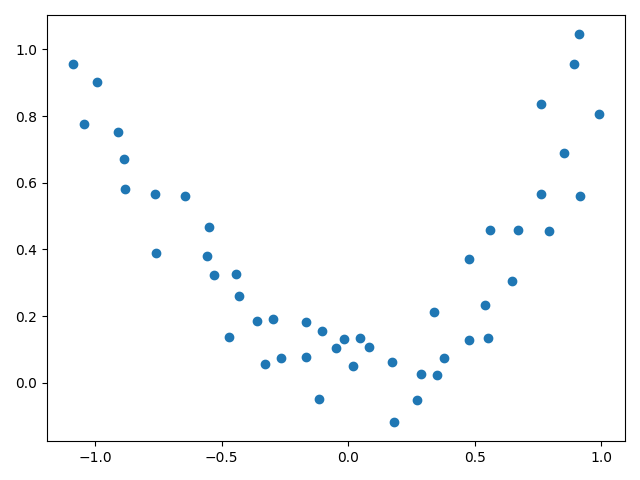
\includegraphics[width=\textwidth]{Images/alpha_1.png}
      \caption{Point set}
      \label{fig:pointset}
    \end{subfigure}
    %%%%%%%%%%%%%%%%
    \begin{subfigure}{0.24\textwidth}
      \centering
      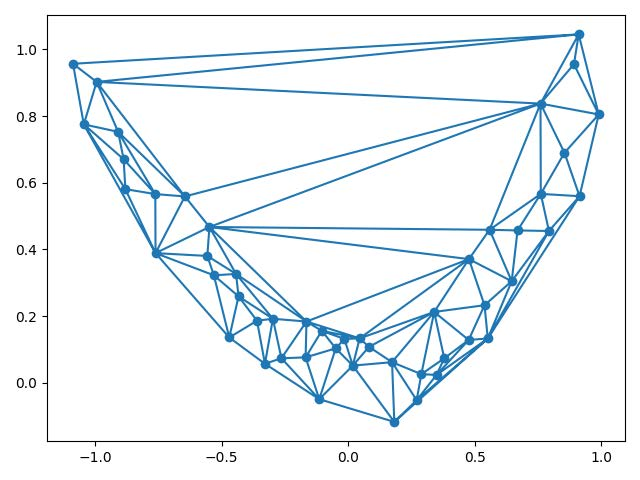
\includegraphics[width=\textwidth]{Images/alpha_2.jpg}
      \caption{Delunay}
      \label{fig:delunay}
    \end{subfigure}
    %%%%%%%%%%%%%%%%
    \begin{subfigure}{0.24\textwidth}
      \centering
      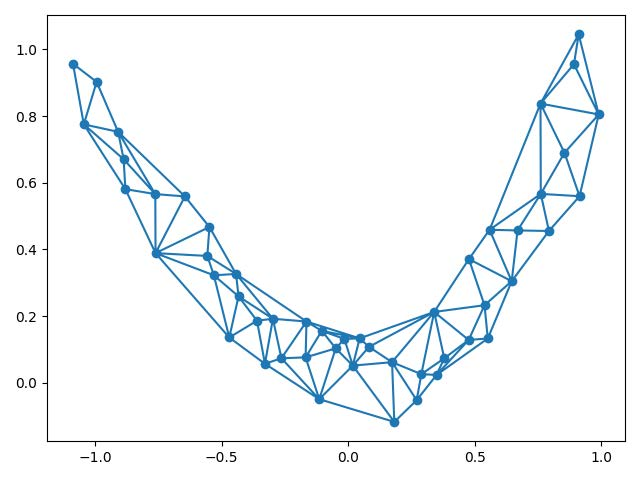
\includegraphics[width=\textwidth]{Images/alpha_3.jpg}
      \caption{\textalpha-complex}
      \label{fig:alphacomplex}
    \end{subfigure}
    %%%%%%%%%%%%%%%%
    \begin{subfigure}{0.24\textwidth}
      \centering
      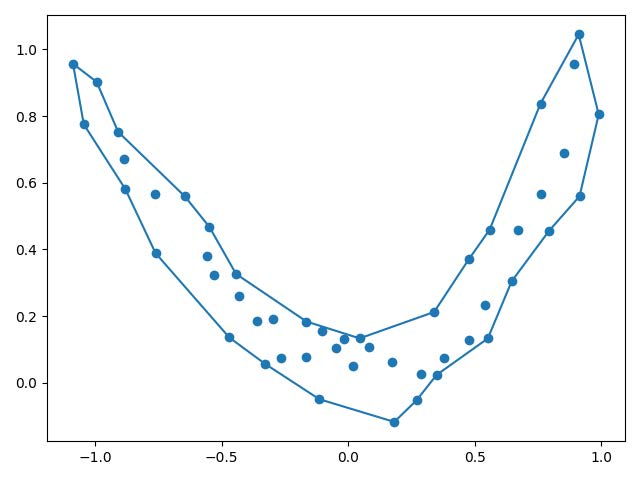
\includegraphics[width=\textwidth]{Images/alpha_4.jpg}
      \caption{\textalpha-shape}
      \label{fig:alphashape}
    \end{subfigure}
  \end{subfigure}
  %%%%%%%%%%%%%%%%
  \caption{\textalpha-shape construction process for the point set of
  \ref{fig:pointset}, with $\alpha = -2.5$. First the Delaunay triangulation is
  built \ref{fig:delunay}, then only triangles whose circumradius is at most
  $-\frac{1}{\alpha}$ are kept, which form a subcomplex called
  \textalpha-complex \ref{fig:alphacomplex}. Finally, the border of the
  \textalpha-complex is the \textalpha-shape \ref{fig:alphashape}.}
  \label{fig:alphabuild}
\end{figure}

The \textalpha-shape is a good representation of the annotated volume, but
because it is a polygonal mesh, it cannot directly be used as a ground truth
segmentation mask for training a neural network. Therefore, the next mandatory
step is voxelization, through which the \textalpha-shape is transformed into
a binary raster volume. The voxelization of a polygonal mesh consists of finding
which cubes (voxels) of a 3-dimensional grid intersect any triangle composing
the mesh: the specific method used to check triangle-cube intersection has been
developed by Voorhies. The final result of the ground truth preprocessing is
illustrated in Fig. \ref{fig:alpha2}.

